\documentclass{beamer}
\usepackage{graphicx} % Required for inserting images

\title{Heuristiken für effiziente Operatorplatzierung in verteilten Stream-Verarbeitungssystemen}
\author{Cedric Sillaber}
\date{June 2024}

\begin{document}

\frame{\titlepage}

\begin{frame}
\frametitle{Inhalt}
\tableofcontents
\end{frame}

\setbeamertemplate{itemize item}{\raisebox{0.1ex}{\scriptsize\textbullet}}
\setbeamertemplate{itemize subitem}{\raisebox{0.1ex}{\scriptsize\textopenbullet}}

\section{Motivation}
\begin{frame}
\frametitle{Motivation}
\begin{itemize}
    \item Verteilte Stream-Verarbeitungssysteme bestehen aus etlichen physischen Rechnern.
    \item Welcher Rechner führt welche Operationen aus?
    \begin{itemize}
        \item Berechnung optimaler Operatorplatzierung ist NP-schwer! \\
        $\rightarrow$ Approximierung durch bekannte Heuristiken
    \end{itemize}
    \item Ziel: Latenz, Netzwerkauslastung, Durchsatz, Verfügbarkeit, etc. minimieren
\end{itemize}
\end{frame}

\section{Operatorplatzierung}
\begin{frame}
\frametitle{Was ist ein Operator?}
\begin{itemize}
    \item Verarbeitungseinheit in einem Stream-Verarbeitungssystem
    \item Beispiele: Filter, Aggregatoren, Joins
\end{itemize}
\begin{center}
    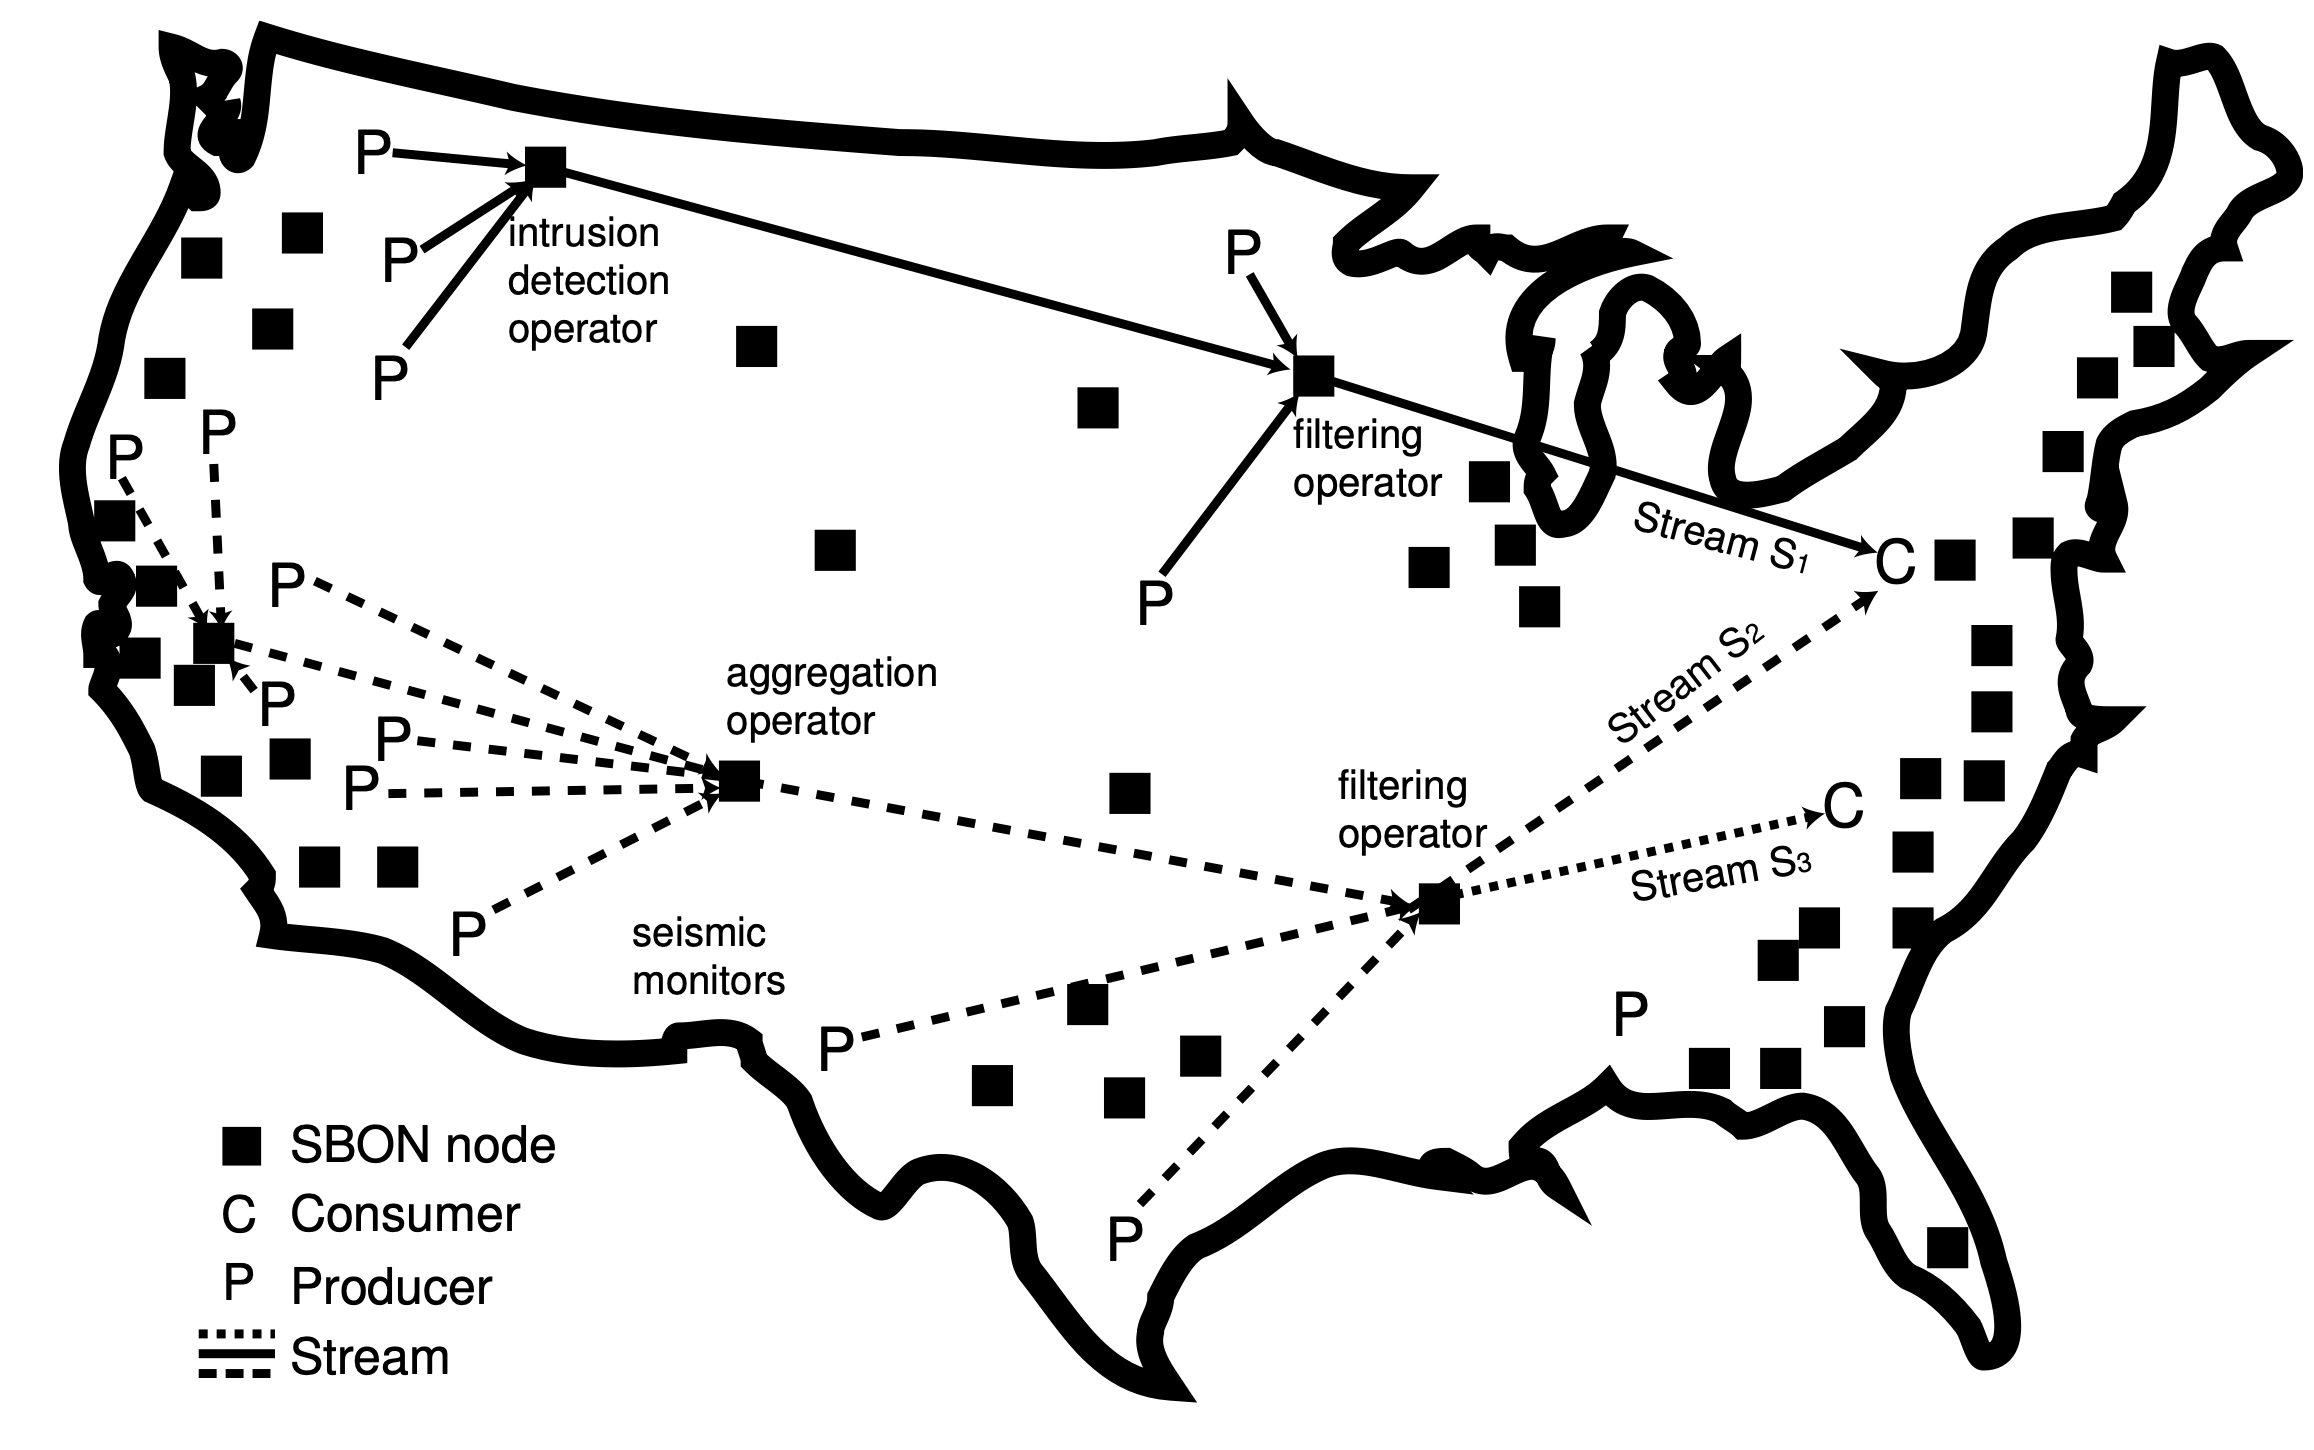
\includegraphics[width=0.6\textwidth]{res/SVS.png}
    % Quelle: Geben Sie hier die Quelle des Bildes an.
\end{center}
\end{frame}

\begin{frame}
\frametitle{Formale Definition von Streamverarbeitungssystemen}
\begin{itemize}
    \item Zwei Modelle, definiert durch gerichtete gewichtete Graphen $G= (V,E)$
    \item \textit{Datenstrom-Modell} beschreibt den Fluss von Datenströmen
    \begin{itemize}
        \item Was sind Quellen, was sind Senken? Wohin fließen Daten?
        \item Wo sollte sortiert, gefiltert, gejoint werden?
        \item Dargestellt mit $G_{svs} = (V_{svs}, E_{svs})$
    \end{itemize}
    \item \textit{Ressourcen-Modell} beschreibt physische Rechner und deren Verknüpfungen
    \begin{itemize}
        \item dargestellt mit $G_{res} = (V_{res}, E_{res})$
    \end{itemize}
\end{itemize}
\end{frame}

\begin{frame}
\frametitle{Problem der Operatorplatzierung}
\begin{itemize}
    \item Mapping zwischen \textit{Datenstrom- } und \textit{Ressourcen-Modell} ($G_{svs}$ und $G_{res}$
\end{itemize}
\begin{center}
    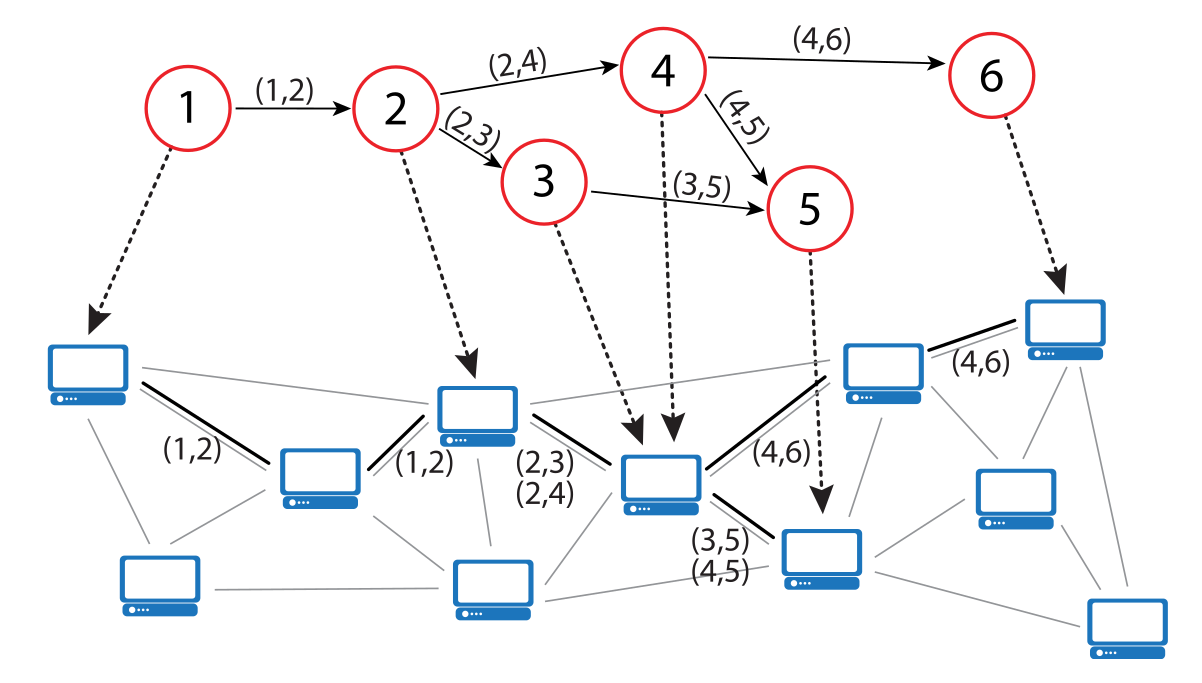
\includegraphics[width=0.6\textwidth]{res/OPP-graph.png}
\end{center}
\end{frame}

\begin{frame}{Formale Definition des OPPs}
\begin{itemize}
    \item kann formal definiert werden als
\end{itemize}
    \[ 
   \begin{gathered}
        \operatorname*{arg\,min}_x F(x) \\
        \sum_{i \in V_{svs}} C_i x_{i,u} < C_u \quad \forall u \in V_{res} \\ % constrain: node resource
        \sum_{u \in V_{res}^i} x_{i,u} = 1 \quad \forall i \in V_{dsp} \\ % constrain: node only placed on candidate resources
        x_{i,u} \in \{0,1\} \quad \forall i \in V_{svs}, u \in V_{res}^i
    \end{gathered} 
    \] 
    \item zu minimierende Funktion $F$:
    \[ 
        \begin{gathered}
            F(x) = w_r \frac{R(x) - R_{min}}{R_{max} - R_{min}} 
            + w_a \frac{log A_{max} - log A(x)}{log A_{max} - log A_{min}} 
            + w_z \frac{Z(x) - Z_{min}}{Z_max - Z_min} 
        \end{gathered}  \label{to-miminize-function}
    \] 
\end{frame}

\section{Heuristiken}
\begin{frame}
\frametitle{Heuristiken}
\begin{itemize}
    \item Näherungsverfahren zur Lösung von Optimierungsproblemen
    \item \textbf{Greedy First-Fit}: 
    \begin{itemize}
        \item Physische Ressourcen basierend auf Straffunktion sortiert (\textit{greedy})
        \item Erster passender Rechner wird ausgewählt und nimmt Operator auf (\textit{first-fit})
        \item Vorteile: Einfachheit, schnelle Berechnungen
        \item Nachteile: Kann in lokalen Optima steckenbleiben
    \end{itemize}
\end{itemize}
\begin{center}
    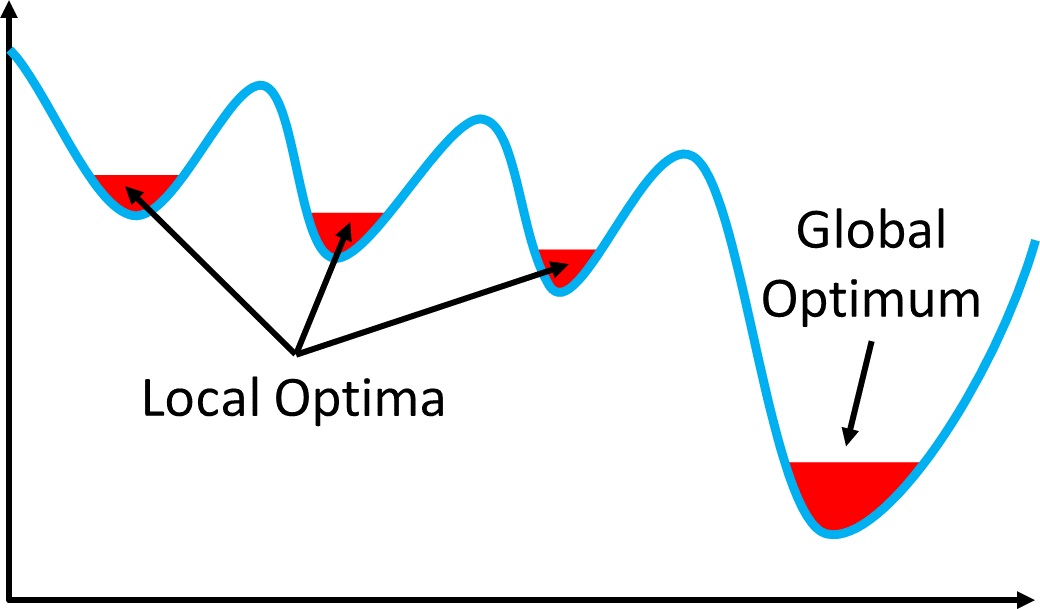
\includegraphics[width=0.5\textwidth]{res/Local-Global-Optimum.png} \\
    \tiny \color{gray} Quelle: https://www.allaboutlean.com/polca-pros-and-cons/local-global-optimum/
\end{center}
\end{frame}

\begin{frame}
\frametitle{Lokale Suche}
\begin{itemize}
    \item Erweiterung von Greedy First-Fit
    \item Ziel: Verbesserung der initialen Lösung
    \begin{itemize}
        \item Verschiebung von Operatoren zwischen Rechnern zur Optimierung
        \item Vermeidung von lokalen Optima
    \end{itemize}
    \item Vorteile: Bessere Lösung als Greedy First-Fit allein
    \item Nachteile: Höherer Berechnungsaufwand
\end{itemize}
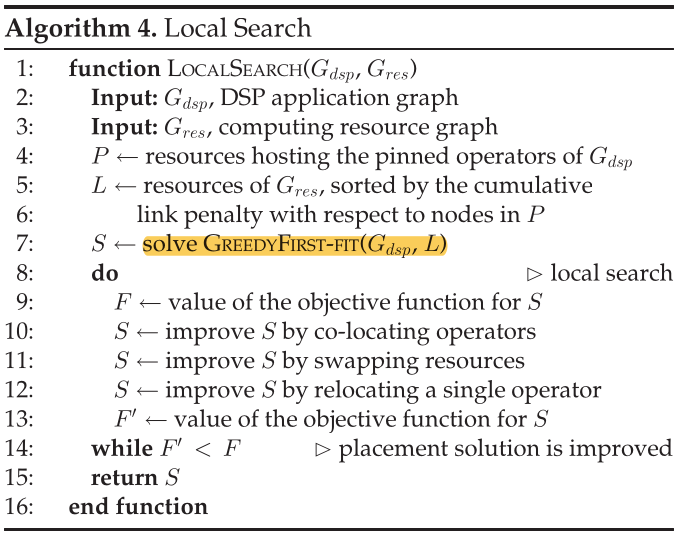
\includegraphics[width=0.5\textwidth]{res/algorithmus-lokale-suche.png} \\
\end{frame}

\begin{frame}
\frametitle{Kombinierte Ansätze}
\begin{itemize}
    \item Aufbauend auf Greedy und Lokaler Suche: Tabu Suche, um Lösungen zu verbessern

\end{itemize}
\end{frame}

\section{Experimentelle Ergebnisse}
\begin{frame}
\frametitle{Experimentelle Ergebnisse}
\begin{itemize}
    \item Vergleich der Heuristiken Greedy First-Fit, Lokaler Suche und Tabu Suche
    \item Metriken: Verfügbarkeit, Netzwerklatenz und Verfügbarkeit
    \item Vergleich von Laufzeit und Beschleunigungsfaktor für drei Topologien
    
\end{itemize}
\vspace{0.3cm}

\end{frame}

\begin{frame}
\frametitle{Vergleich der Heuristiken}
\begin{center}
    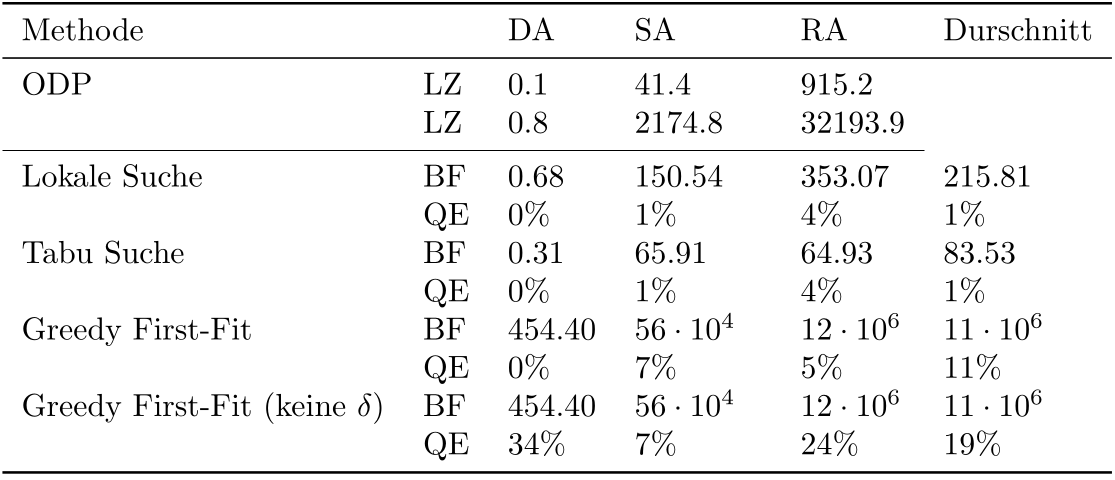
\includegraphics[width=0.8\textwidth]{res/evaluation.png} 
\end{center}
\begin{itemize}
    \item Optimale Lösung benötigt 8h, Greedy First-Fit Bruchteil einer Sekunde.
    \item Kompromiss zwischen Qualität und Lafzeit

\end{itemize}
\end{frame}

\section{Fazit}
\begin{frame}
\frametitle{Fazit}
\begin{itemize}
    \item Greedy First-Fit, Lokale Suche und Tabu Suche bieten effiziente Lösungen für das Operatorplatzierungsproblem.
    \begin{itemize}
        \item Greedy First-Fit: schnelle, aber minderwertige Lösungen.
        \item Lokale Suche und Tabu Suche: qualitativ besser, aber zeitintensiver.
    \end{itemize}
    \item Alle Heuristiken zeigten eine deutliche Verkürzung der Laufzeit im Vergleich zur optimalen Lösung.
\end{itemize}
\end{frame}

\begin{frame}
\frametitle{Zukunftsaussichten}
\begin{itemize}
    \item Entwicklung komplexerer Heuristiken zur besseren Approximation des OPP-Problems.
    \item Fokussierung auf zur Laufzeit anpassbare Heuristiken für dynamische Bedingungen.
    \item Analyse der erneuten Konfiguration während der Laufzeit für Big Data-Anwendungen.
\end{itemize}
\end{frame}
\end{document}
